\documentclass{article}

\usepackage{graphicx}
\usepackage{tikz}
\usepackage{tikzsymbols}
\usetikzlibrary{calc,patterns,shapes.geometric}
\pagestyle{empty}
\usepackage[margin=0pt]{geometry}
\geometry{papersize={14in,12in}}

\def\centerarc[#1](#2)(#3:#4:#5){\draw[#1] ($(#2)+({#5*cos(#3)},{#5*sin(#3)})$) arc (#3:#4:#5);}

\begin{document}
	\begin{figure}
		\centering
		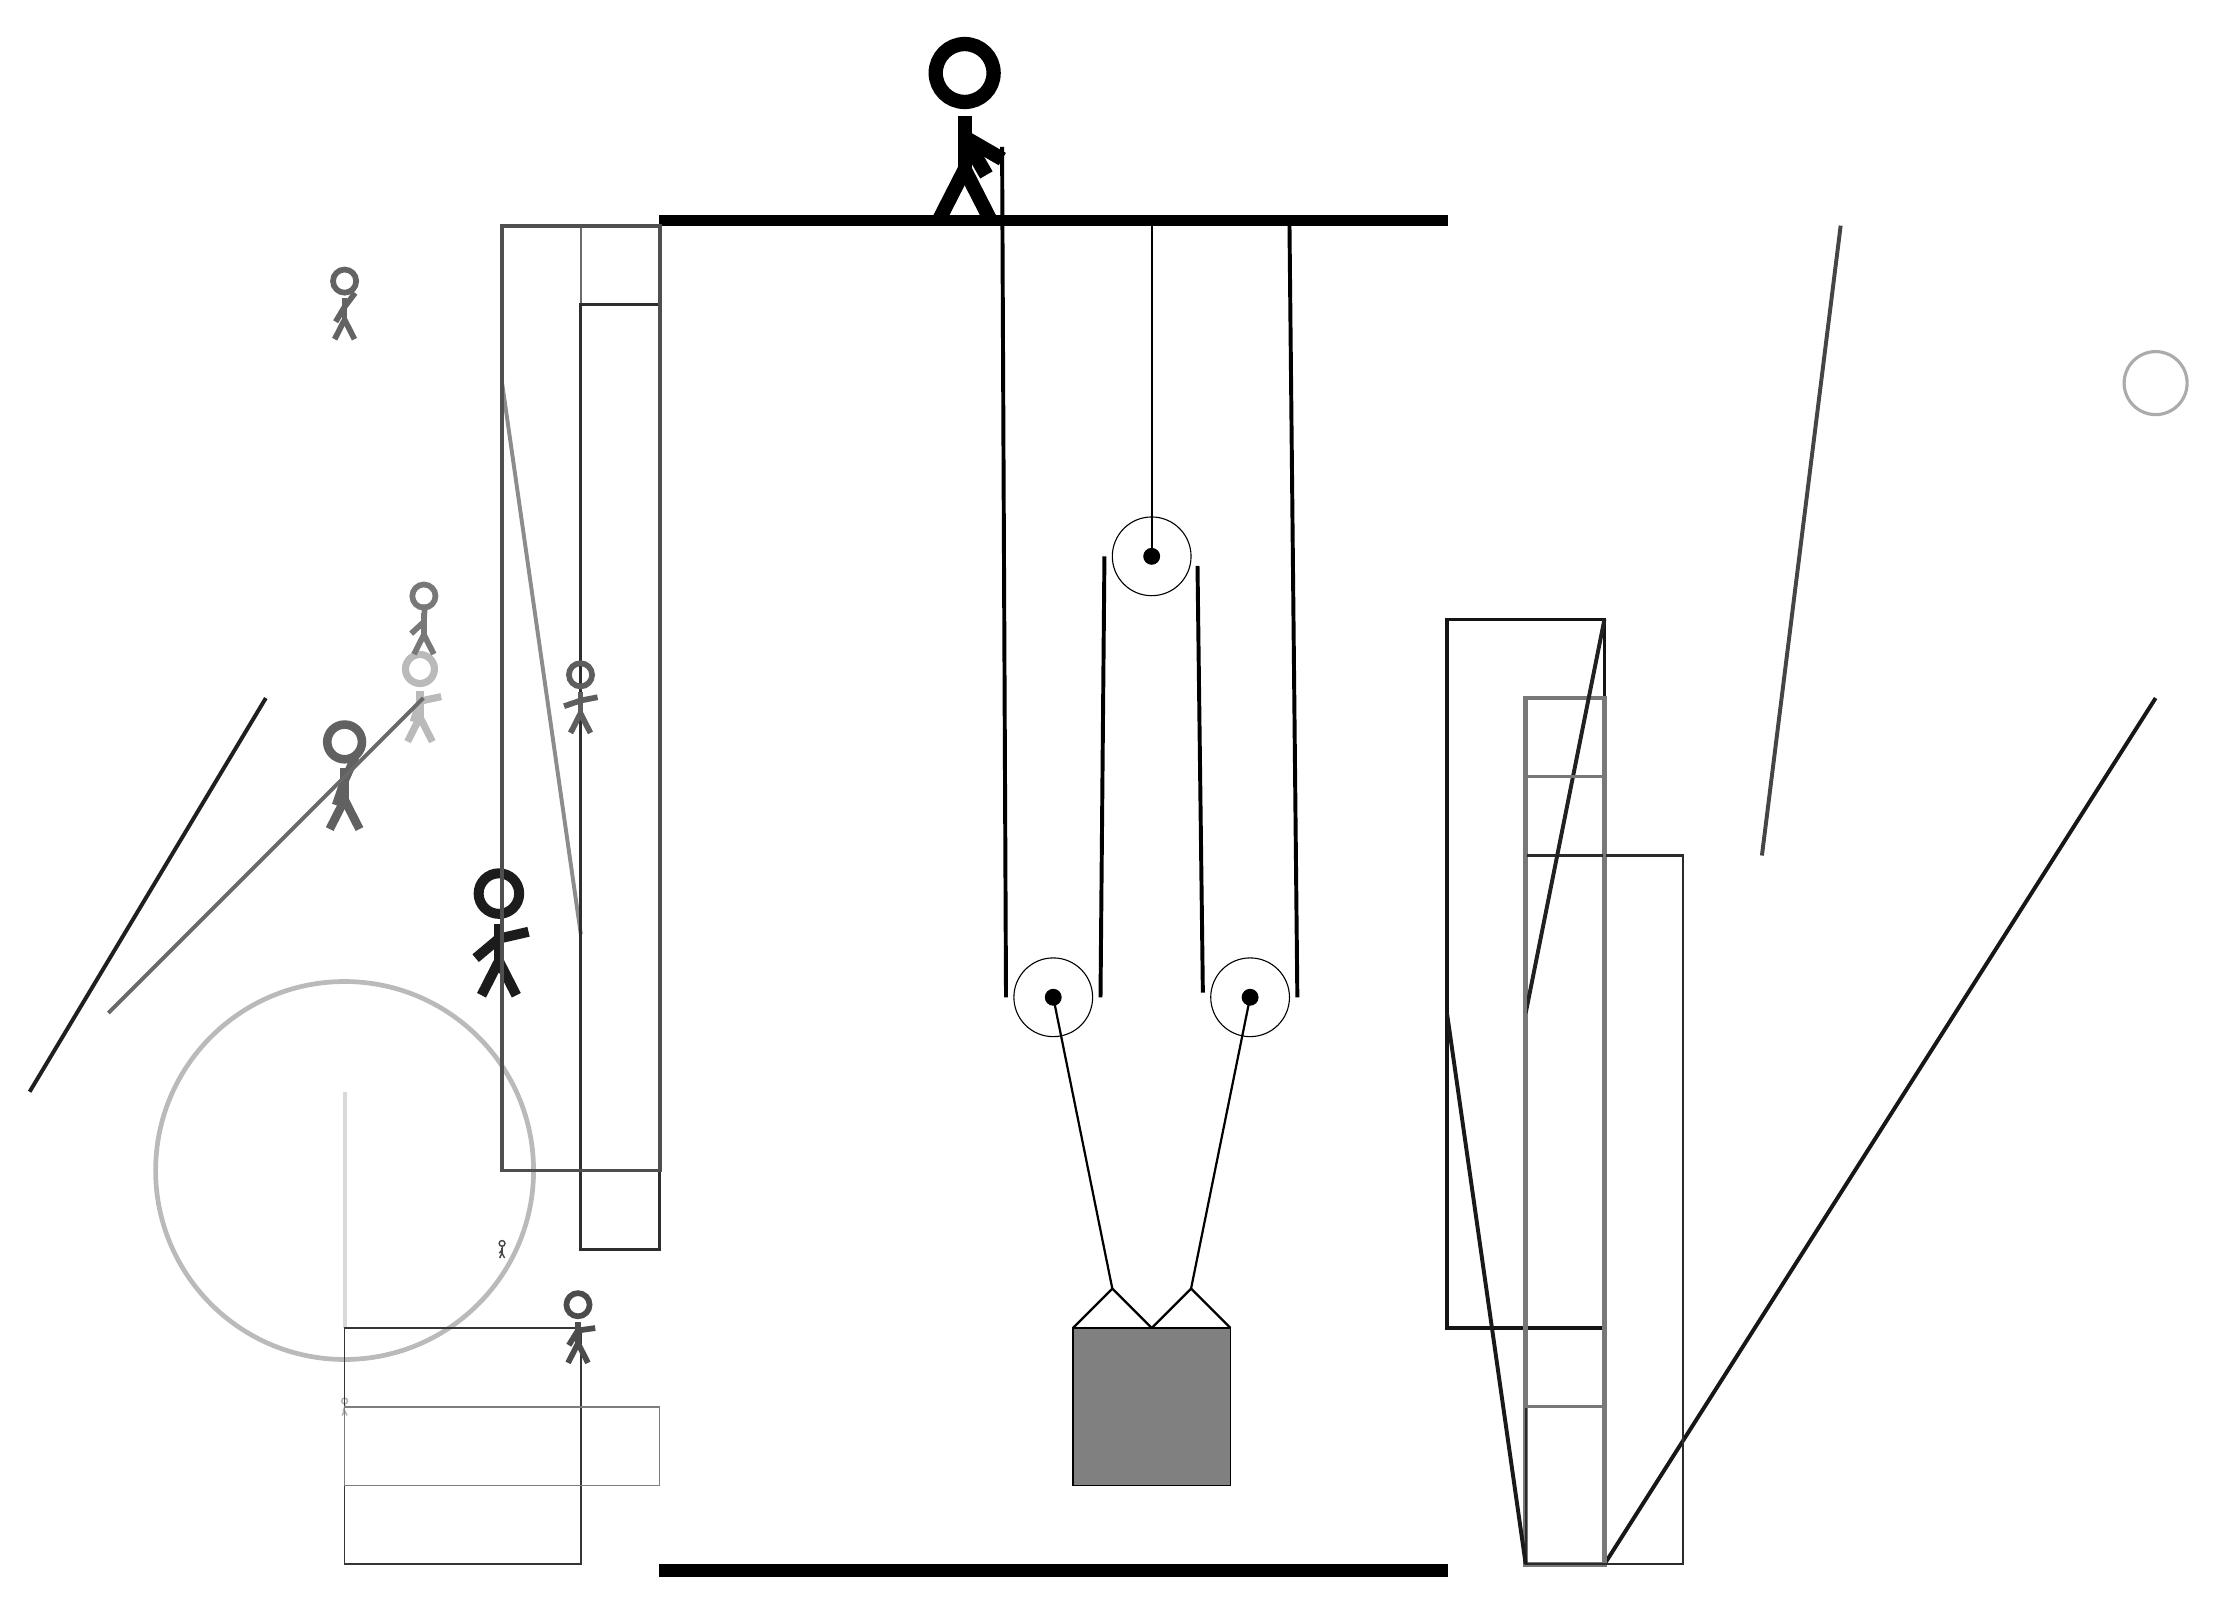
\begin{tikzpicture}
			%%%%% START %%%%%
			
			\draw[fill=black] (-4, 14) rectangle (6, 14.125);
			
			\draw (1, 4.2) circle (0.5);
			\draw[fill=black] (1, 4.2) circle (0.1);
			
			\draw (2.25, 9.8) circle (0.5);
			\draw[fill=black] (2.25, 9.8) circle (0.1);
			\draw[thick] (2.25, 9.8) -- (2.25, 14);
			
			\draw (3.5, 4.2) circle (0.5);
			\draw[fill=black] (3.5, 4.2) circle (0.1);
			
			\draw[thick] (3.5, 4.2) -- (2.75, 0.5);
			\draw[thick] (1, 4.2) -- (1.75, 0.5);
			\draw[thick]  (1.25, 0) -- (1.75, 0.5) -- (2.25, 0);
			\draw[thick]  (2.25, 0) -- (2.75, 0.5) -- (3.25, 0);
			\draw[fill=black!50] (1.25, 0) rectangle (3.25, -2);
			
			\draw[line width=0.5mm] (0.35, 15) --  (0.4, 4.2);
			\centerarc[line width=0.5mm](1, 4.2)(180:360:0.6);
			\draw[line width=0.5mm] (1.6, 4.2) -- (1.65, 9.8);
			\centerarc[line width=0.5mm](2.25, 9.8)(-20:180:0.6);
			\draw[line width=0.5mm](2.832, 9.68) -- (2.9, 4.26);
			\centerarc[line width=0.5mm](3.5, 4.2)(160:360:0.6);
			\draw[line width=0.5mm](4.1, 4.2) -- (4.0, 14);
			
			\node at (-0.07, 15.2) {\Strichmaxerl[10][120][-30]};
			
			\node[line width=0.5mm, color=black!31] at (-8, -1) {\Strichmaxerl[1][68][84]};
			
			\node[line width=0.2mm, color=black!62] at (-8, 7) {\Strichmaxerl[6][71][66]};
			\draw[line width=0.5mm, color=black!45](-5, 5) -- (-6, 12);
			\draw[line width=0.4mm, color=black!92] (8, 9) rectangle (6, 0);
			\draw[line width=0.5mm, color=black!91](8, -3) -- (15, 8);
			\node[line width=0.4mm, color=black!72] at (-6, 1) {\Strichmaxerl[1][51][85]};
			
			\draw[line width=0.6mm, color=black!53] (7, 8) rectangle (8, -3);
			\draw [line width=0.6mm, color=black!27](-8, 2) circle (2.4);
			\draw [line width=0.4mm, color=black!33](15, 12) circle (0.4);
			
			\draw[line width=0.5mm, color=black!88](-9, 8) -- (-12, 3);
			
			\draw[line width=0.5mm, color=black!15](-8, 3) -- (-8, 0);
			\draw[line width=0.2mm, color=black!79] (-5, -3) rectangle (-8, 0);
			\draw[line width=0.3mm, color=black!58] (-5, 14) rectangle (-5, 13);
			\node[line width=0.7mm, color=black!27] at (-7, 8) {\Strichmaxerl[5][72][12]};
			\draw[line width=0.3mm, color=black!83] (7, 6) rectangle (9, -3);
			\draw[line width=0.4mm, color=black!82] (-5, 1) rectangle (-4, 13);
			\node[line width=0.2mm, color=black!89] at (-6, 5) {\Strichmaxerl[7][40][13]};
			
			\draw[line width=0.5mm, color=black!59](-7, 8) -- (-11, 4);
			\draw[line width=0.5mm, color=black!73](10, 6) -- (11, 14);
			\draw[line width=0.5mm, color=black!87](8, 9) -- (7, 4);
			\node[line width=0.3mm, color=black!53] at (-7, 9) {\Strichmaxerl[4][43][87]};
			
			\node[line width=0.3mm, color=black!70] at (-5, 0) {\Strichmaxerl[4][58][8]};
			\node[line width=0.2mm, color=black!63] at (-5, 8) {\Strichmaxerl[4][19][11]};
			\node[line width=0.4mm, color=black!61] at (-8, 13) {\Strichmaxerl[4][59][53]};
			\draw[line width=0.5mm, color=black!90](7, -3) -- (6, 4);
			\draw[line width=0.4mm, color=black!53] (8, -1) rectangle (7, 7);
			\draw[line width=0.2mm, color=black!51] (-4, -2) rectangle (-8, -1);
			\draw[line width=0.5mm, color=black!69] (-6, 14) rectangle (-4, 2);
			
			\draw[fill=black] (-4, -3) rectangle (6, -3.15);
			
			%%%%% END %%%%%
		\end{tikzpicture}
	\end{figure}	
\end{document}